\documentclass[conference]{IEEEtran}
\IEEEoverridecommandlockouts

\usepackage{cite}
\usepackage{amsmath,amssymb,amsfonts}
\usepackage{algorithm}
\usepackage{algorithmic}
\usepackage{graphicx}
\usepackage{textcomp}
\usepackage{xcolor}
\usepackage{booktabs}
\usepackage{url}

\graphicspath{{images/}}

\begin{document}

\title{Learn Only What You Can Verify: Hardening the Label Channel of Online IoT DDoS Detectors}

\author{\IEEEauthorblockN{Shirish Giroti}
\IEEEauthorblockA{Dept.\ of Computer Science and Engineering\\
IIITDM Kancheepuram\\
Roll No.\ CS23B2041\\
Email: cs23b2041@iiitdm.ac.in}}

\maketitle

\begin{abstract}
Online Internet of Things (IoT) Distributed Denial of Service (DDoS) detectors
are often presented as robust to evasion because they keep adapting to
streaming traffic. This paper challenges that assumption. We re-evaluate the
Multi-Stage Adversarial Defense (MSAAD), a representative online framework, on
IoTID20, CICIoT2023 and a time-ordered CIC-IDS2017 stream, using 15 random seeds
and paired statistical tests. We find that MSAAD's resilience depends on an
instant, correct label channel: evasion stays at or below 0.12\% with immediate
labels, but rises to 17--49\% for valid-traffic transfer attacks when labels are
removed, and a delay of 5{,}000 flows already lets 9--28\% of attack traffic
through. Label poisoning takes over the online learner, raising evasion to
99.7--99.96\%, while MSAAD's own filter catches only 11--17\% of valid
adversarial flows on IoTID20. To close this gap, we propose verified-label
learning with uncertainty-directed audits under a 10\% budget. It keeps evasion
at or below 1.2\% under full label poisoning on all three datasets and cuts
false alarms under attack by 8--13$\times$ compared with random audits.
Finally, we show that trusting attack labels opens a framing attack. Under
combined poisoning and framing, importance-weighted consensus updates with
uncertainty-directed audits keep evasion at or below 0.65\% when the attacker
also perturbs its traffic, and at or below 1.7\% when it does not, at the cost
of 2--26\% false alarms.
\end{abstract}

\begin{IEEEkeywords}
Online intrusion detection, IoT DDoS detection, adversarial machine learning,
data poisoning, label noise, active learning, concept drift.
\end{IEEEkeywords}

\section{Introduction}\label{sec:intro}

The growth of IoT over the past decade has brought significant developments
in modern digital infrastructure. IoT networks are the foundation for
self-monitoring systems in manufacturing, automated crop telemetry, and smart
city frameworks, speeding up technological progress by leaps and bounds. IoT
has bridged the gap between the physical and digital worlds, bringing real-time
data visibility, efficiency, and predictive analytics.

But the higher the mountain, the longer its shadow: the same connectivity
that makes IoT useful also exposes it. IoT networks have many
vulnerabilities waiting to be exploited by different types of attackers. For
example, IoT botnets such as Mirai exploit vulnerable edge devices to
orchestrate massive DDoS attacks~\cite{kolias2017mirai} that overwhelm network
resources.

While standard ML detectors achieve high accuracy in static, offline settings,
real-world IoT traffic exhibits continuous concept drift, causing static models
to lose accuracy over time. As a result, recent DDoS detection research is
shifting towards online learning detectors that update in real time without
full retraining~\cite{beshah2024drift,yang2021pwpae}.
A frozen detector, once evaded, stays evaded; an online detector can recover,
but only if the labels it learns from are correct.

As a representative baseline of recent online defenses, Beshah et
al.~\cite{beshah2025msaad} introduced the Multi-Stage Adversarial Defense
(MSAAD) framework for online IoT DDoS detection, a three-layer architecture
described in Section~\ref{sec:related}. Evaluated on the IoTID20 and CICIoT2023
datasets, MSAAD reports a clean classification accuracy of 99.50\% and 99.28\%,
respectively. While accuracy degrades to 38.92--67.12\% on IoTID20 and
13.08--32.38\% on CICIoT2023 under gradient-based evasion attacks (FGSM, BIM,
PGD, C\&W), the authors report that the RADP layer restores detection accuracy
to roughly 99\%.

Despite these figures, a methodological audit reveals three gaps that obscure
real-world deployment performance:
\begin{enumerate}
\item \textit{Instant ground-truth labels.} MSAAD's prequential protocol
assumes that the true label $y_i$ of every flow arrives instantly after
prediction (Algorithm~1, line~13). Since the system gets instant and accurate
labels, it is never tested against real-world issues like delayed or tampered
labels. It only seems resilient because it quickly adapts to attack patterns
after seeing a few flows.
\item \textit{Unconstrained, all-flow perturbations.} These attacks modify
scaled features without domain checks, so some resulting flows could not exist
as real network traffic, such as negative values or a Min greater than the
Mean. The method also perturbs benign flows, which artificially degrades
precision. A real-world adversary only controls its own traffic.
\item \textit{Missing security metrics.} MSAAD relies on overall accuracy,
which is misleading under IoT class imbalance, where always predicting DDoS
already yields high accuracy. It omits the false-positive rate (FPR), the
operational burden on legitimate traffic, and the attack success rate (ASR),
which measures evasion directly.
\end{enumerate}

The gaps noticed in the existing defences give rise to a fundamental question:
``What happens to an online detector when its labels are not instant and
correct?'' An online detector is only as robust as its label channel, meaning
it should learn only what it can verify and direct verification precisely where
it is unsure. We address this by treating the label channel explicitly as an
attack surface and evaluating MSAAD against late, missing, poisoned and framed
label streams. We then propose verified-label learning, where our learner never
learns an unverified benign label, re-weights audited benign flows, and accepts
an unverified DDoS label only when the detector agrees, allocating a 10\% audit
budget to the flows with the highest prediction uncertainty. We evaluate this
approach on IoTID20~\cite{ullah2020iotid20}, CICIoT2023~\cite{neto2023ciciot}
and a time-ordered, corrected CIC-IDS2017~\cite{engelen2021troubleshooting}
using 15 seeds and Holm-corrected paired statistical tests. Our contributions
are:
\begin{enumerate}
\item We define a threat model that incorporates the label channel and
re-evaluate MSAAD, showing that evasion remains $\le 0.12\%$ under instant
labels, rises to 17--49\% with no labels, and reaches 9--28\% when labels are
delayed by 5{,}000 flows.
\item Through a corrected evaluation that restricts attack perturbations to
valid traffic and reports FPR and ASR, we show that label poisoning drives the
learner to 99.7--99.96\% evasion, while MSAAD's RADP filter detects only
11--17\% of valid attacks on IoTID20.
\item We propose verified-label learning combined with uncertainty-directed
audits, checked at matched detection rates, which restricts evasion to
$\le 1.2\%$ under full label poisoning while achieving an FPR under attack
8--13$\times$ lower than with random audits.
\item We identify framing as an availability attack created by blindly trusting
DDoS labels, and show that under simultaneous poisoning and framing, evasion
remains $\le 1.7\%$ at a cost of 2--26\% false alarms. We also document
negative results for RADP, adversarial training (which halts transfer but
doubles FPR), and a graph-based detection stage.
\end{enumerate}

\section{Background and Related Work}\label{sec:related}

\subsection{The Base System}
Beshah et al.~\cite{beshah2025msaad} recently introduced the Multi-Stage
Adversarial Defense (MSAAD) framework for online DDoS detection in IoT
networks. The architecture builds on their earlier drift-adaptive
ensemble~\cite{beshah2024drift} by chaining three modules. First, a GAN-based
Resilient Adversarial Detection and Purification (RADP) filter detects
adversarial flows and deletes them before classification. Second, a pool of
five drift-aware online learners classifies the remaining flows. Finally, a
multi-armed bandit using Thompson sampling (MABTSE) selects the top three
learners for each flow and combines their outputs with an accuracy-update weighted probability
averaging ensemble (AUWPAE). The authors report post-defence accuracies of roughly 99\%
on public benchmarks, but their evaluation rests on two unstated choices that we
examine in Section~\ref{sec:threat}: ground-truth labels arrive immediately, and
the attacker perturbs every flow without domain constraints.

\subsection{Online Detection and Concept Drift}
Online network intrusion detection needs streaming algorithms that process
continuous traffic within tight memory limits. Adaptive classifiers such as
Adaptive Random Forests (ARF)~\cite{gomes2017arf} and Streaming Random Patches
(SRP)~\cite{gomes2019srp} handle drift by embedding explicit drift detectors
such as ADWIN~\cite{bifet2007adwin} or DDM~\cite{gama2004ddm}.
Performance-weighted ensembles such as PWPAE~\cite{yang2021pwpae} combine such
learners, and libraries such as River~\cite{montiel2021river} implement them.
Unsupervised pipelines such as Kitsune~\cite{mirsky2018kitsune} avoid labels by
flagging anomalies, and CADE~\cite{yang2021cade} detects and explains drifting
samples in security data. Delayed-label
protocols~\cite{grzenda2020delayed,ceschin2024stream} model realistic feedback
lag, but they assume the late feedback is still correct. Our work treats the
label feedback loop itself as an attack surface exposed to delay, poisoning and
framing.

\subsection{Realistic Evasion of Network Detectors}
Evasion attacks commonly use gradient methods such as
FGSM~\cite{goodfellow2015fgsm}, BIM~\cite{kurakin2017bim} and
PGD~\cite{madry2018pgd}, optimisation-based attacks such as
C\&W~\cite{carlini2017cw}, or decision-based queries such as
HopSkipJump~\cite{chen2020hsj}. Applied to network intrusion detection, feature
perturbations must respect domain constraints; otherwise, the resulting traffic
could not exist~\cite{pierazzi2020problemspace}. Realistic adversaries can also
manipulate only their own traffic~\cite{apruzzese2022realistic}, and
methodology guidelines warn against judging detectors by overall accuracy under
severe class imbalance~\cite{arp2022dosanddonts}. Our evaluation therefore
perturbs attack flows only, repairs every adversarial flow to valid traffic, and
reports the attack success rate (ASR) and false-positive rate (FPR).

\subsection{Poisoning, Label Noise and Trusted Labels}
Data poisoning attacks corrupt a model by manipulating its training data, from
crafted points against support vector machines~\cite{biggio2012poisoning} to
attacks on online learners as they update~\cite{zhang2020online}. In network
security, attackers can plant clean-label backdoors in batch-trained flow
classifiers~\cite{severi2023poisoning}. Older attacks on signature learners
mislead the learner with crafted samples
(Paragraph~\cite{newsome2006paragraph}) or trick it into signatures that block
legitimate traffic (Allergy~\cite{chung2006allergy}); the latter is a precursor
of the framing attack we study. Defences against label noise include Gold Loss
Correction (GLC), which uses a small trusted set~\cite{hendrycks2018glc}, and
active learning~\cite{settles2009active}, which spends a labelling budget on
informative samples; importance-weighted active learning (IWAL) keeps such
sampling unbiased~\cite{beygelzimer2009iwal}, and Lin et al.\ study active
learning under malicious mislabelling on image data~\cite{lin2021activelearning}.
Our strategy brings these ideas into an online NIDS: we combine trusted audits,
fixed-count duplication of audited benign flows, and uncertainty-directed audits
to limit label delay, poisoning and framing together.

\subsection{Defences and Adaptive Attacks}
Detect-and-reject defences often collapse against adaptive
attackers~\cite{tramer2020adaptive} or rely on obfuscated
gradients~\cite{athalye2018obfuscated}, so evaluation guidelines call for
testing each defence against attacks tailored to it~\cite{carlini2019evaluating};
adversarial training~\cite{madry2018pgd} remains the standard baseline. We test
the RADP filter against domain-constrained attacks it was not tuned for, and
compare adversarial training against label-only HopSkipJump attacks.

\subsection{Graph and Temporal Detectors}
Graph-based intrusion detectors build relational structures over flow
endpoints, using graph neural networks such as
E-GraphSAGE~\cite{lo2022egraphsage}, temporal graph models in which simple
MLP-based designs can match complex ones~\cite{cong2023graphmixer}, or streaming
edge counters such as MIDAS~\cite{bhatia2020midas}. In our detector chain, a
host-graph GNN does not outperform a parameter-matched MLP.

We are not aware of prior work that evaluates an online IoT DDoS detector's
label channel under simultaneous delay, poisoning and framing, or that defends
it with verified-label learning.

\section{System and Threat Model}\label{sec:threat}

\subsection{The Online Detector and Its Label Channel}
Our online detector runs a prequential (test-then-train) streaming loop
(Fig.~\ref{fig:system}): it classifies each incoming flow $x_t$ and then learns
from a label $l_t$ supplied by a labeller. In real deployments, these labels
come from signature rules, analyst triage, threat-intelligence feeds, or the
model's own earlier predictions. Rule latency, stale feeds and low-rate evasion
mean that labels are often delayed, missing, or wrong. To verify uncertain
traffic, the defender can spend an audit budget of $a = 10\%$ of flows on
forensic checks or an expert verifier, which returns the true label $y_t$.
MSAAD uses a vanilla update policy that trains on every incoming label
immediately, without verification (Algorithm~1, line~13); our approach instead
filters the labels through a verified-label update policy.

\begin{figure}[t]
\centering
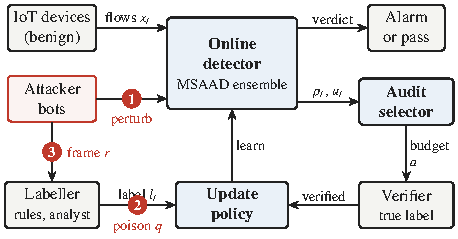
\includegraphics[width=\columnwidth]{fig_system.pdf}
\caption{System overview. The online detector classifies each flow $x_t$; the audit selector uses the uncertainty $u_t$ and the budget $a$ to send some flows to the verifier, and the update policy decides which labels the detector learns from. Numbered circles mark the attacker's three entry points: (1) perturbation of its own flows, (2) label poisoning with rate $q$, and (3) framing with rate $r$.}
\label{fig:system}
\end{figure}

\subsection{Attacker Goals, Knowledge and Capabilities}
We model a grey-box adversary with two goals: evasion (G1), getting DDoS flows
past the detector, measured by the attack success rate (ASR); and availability
disruption through framing (G2), getting benign flows flagged as DDoS, measured
by the false-positive rate (FPR) on genuine benign flows. The attacker knows the
feature space and trains a local surrogate on similar IoT traffic, but cannot
access the detector's weights or its audit selection. It has three
capabilities. First, it can perturb its own attack flows within an $L_\infty$
bound of $\epsilon = 0.1$ on scaled features, provided the result remains valid
traffic. Second, it can cause the labeller to mark each of its flows benign
with probability $q$ (label poisoning). Third, it can frame benign traffic: its
hosts send benign-looking flows at a rate of $r$ per test flow, which the
labeller correctly marks as DDoS because they come from attacker hosts.
Independently of the attacker, labels may also arrive late by a fixed number of
flows or seconds.

In a live deployment, an attacker raises $q$ by exploiting blind spots in
rule-based and self-labelling systems. Low-rate or pulsed floods stay below volume thresholds, avoiding alerts and
getting labelled benign by default~\cite{zhang2020online}. Attackers can also
rotate or spoof source IPs to bypass standard threat blocklists. In
self-labelling systems the problem escalates, as every successful evasion gets
learned as a benign training sample. This is made worse by the fact that
security data streams often have late or noisy labels
anyway~\cite{grzenda2020delayed,ceschin2024stream}. While $q = 1$ is the worst
case, real levels depend on the labelling infrastructure, so we test
$q \in \{0, 0.1, 0.25, 0.5, 1\}$.

\subsection{Out of Scope}
We do not consider direct compromise of the audit verifier, attacks on the
feature extractor, or packet-level replay. A more adaptive adversary could also
shape its poisoned or framing flows to avoid uncertainty-directed audits;
attacks that steer uncertainty-based selection exist in other
domains~\cite{zhi2025ala}. We treat this as an open threat and return to it
among the limitations in Section~\ref{sec:discussion}.

\section{Methodology}\label{sec:method}

\subsection{Datasets and Stream Protocol}
We evaluated our framework on three network intrusion datasets, summarized in
Table~\ref{tab:datasets}: IoTID20~\cite{ullah2020iotid20},
CICIoT2023~\cite{neto2023ciciot}, and the corrected version of
CIC-IDS2017~\cite{sharafaldin2018cicids,engelen2021troubleshooting}. From
IoTID20 we used normal traffic and the Mirai UDP, HTTP and ACK floods; we
excluded brute-force flows because they are not DDoS. This data keeps its
published file order and has 79 features. From CICIoT2023 we used one CSV part
with benign traffic and all DDoS classes, 46 features, in file order. Because
neither benchmark is truly time-ordered, we also used the Friday capture of the
corrected CIC-IDS2017 (20:31--21:26 on the file clock) as a strictly
time-ordered stream.

Each run used 30{,}000 evenly spaced flows. The first 20{,}100 (67\%) trained
the detector, and the remaining 9{,}900 formed the prequential
(predict-then-learn) test stream. DDoS flows make up 87.6\%, 96.6\% and 75.4\%
of the test streams of IoTID20, CICIoT2023 and CIC-IDS2017. To prevent leakage,
a running min-max scaler transforms each flow before the model learns from it,
and IP addresses and timestamps are never used as features.

Two dataset caveats shape these experiments. First, IoTID20's file order is
only about 50\% time-ordered, and all its benign flows come from the first
capture week, so any drift it shows is an artefact rather than a real traffic
shift. Second, CICIoT2023 has only about 330 benign test flows, so a single
misclassified flow moves the false-positive rate (FPR) by about 0.3 points.

\begin{table}[t]
\caption{The three streams and how they were built. Feat.: number of features; Order: file order or time order; DDoS (test): share of DDoS flows in the 9{,}900-flow test stream.}
\label{tab:datasets}
\centering
\footnotesize
\setlength{\tabcolsep}{3pt}
\begin{tabular}{@{}p{1.55cm}p{3.15cm}ccc@{}}
\toprule
Dataset & Classes used & Feat. & Order & DDoS (test) \\
\midrule
IoTID20 & Normal; Mirai UDP, HTTP and ACK floods & 79 & file & 87.6\% \\
CICIoT2023 & Benign; DDoS-* (one CSV part) & 46 & file & 96.6\% \\
CIC-IDS2017 (corrected) & Friday BENIGN and DDoS, 20:31--21:26 & 79 & time & 75.4\% \\
\bottomrule
\end{tabular}
\end{table}

\subsection{Detector Reimplementation}
Because no source code was released, we reimplemented layers 2 and 3 of MSAAD
from scratch with the River 0.22 library~\cite{montiel2021river}. The
classifier pool has five online learners: Adaptive Random Forest with ADWIN
(ARF-ADWIN), ARF with DDM (ARF-DDM), Streaming Random Patches with ADWIN
(SRP-ADWIN), SRP with DDM (SRP-DDM), and $k$-nearest neighbours with ADWIN
(KNN-ADWIN). Following the base paper, the ARF models use 3 trees, the SRP
models 3 base learners, and KNN-ADWIN uses $k=5$ over a window of 100 flows.

A Thompson-sampling bandit~\cite{chapelle2011thompson} with Beta(1,1) priors
selects the top three learners for each flow, and AUWPAE combines their outputs
with weights $1/(\mathrm{MSE}_j + 10^{-4})$, where $\mathrm{MSE}_j$ is learner
$j$'s error over the last 500 flows. The base paper leaves two details open, so
we made two assumptions: the bandit's reward is each learner's correctness on
every flow, and KNN-ADWIN was rebuilt to fit River 0.22.

\subsection{Attacks and Feasibility Repair}\label{sec:attacks}
For the grey-box threat, we trained an MLP surrogate on the training split. It
generated FGSM, BIM, PGD and C\&W attacks with $\epsilon = 0.1$ on scaled
features. We only perturbed DDoS flows, unlike MSAAD, which changes benign
traffic too. To fix impossible features, we mined rules from clean dataset
flows (constant, binary, categorical, integer and non-negative features, equal
groups, and $\mathrm{Min} \le \mathrm{Mean} \le \mathrm{Max}$). The repair step
pushes each adversarial flow back inside these rules without increasing any
single feature's perturbation. We report both raw and repaired results.
Finally, we tested decision-based adaptive attackers using
HopSkipJump~\cite{chen2020hsj} with 2{,}000 queries per flow.

\subsection{Label Feedback Modes}
We evaluated five feedback modes. \textit{Instant} feedback follows the base
paper: the true label arrives right after each prediction (Algorithm~1,
line~13). \textit{None} (frozen) means the detector receives no updates during
the test stream. \textit{Flow-delayed} feedback holds back each label by 1{,}000
or 5{,}000 flows. \textit{Time-delayed} feedback holds labels back by 60 or
300~seconds; it runs only on the timestamped CIC-IDS2017 stream. Finally, with
\textit{self-labelling} the detector learns from its own earlier verdicts.

\subsection{Update Policies}
We compared several update policies, formalized in
Algorithm~\ref{alg:policy}. \textit{Vanilla} updates the model on every
incoming label without checking it, as MSAAD does. \textit{Audit} uses verified
labels only to update the Thompson-sampling selector and leaves the learners
unchanged. \textit{Guard} checks suspicious benign labels before allowing an
update, while \textit{Strict} never learns an unverified benign label: only
audited benign flows are learned.

\textit{IW-strict} also duplicates each audited benign flow
$c = \min(\mathrm{round}(1/a), 20)$ times, which gives $c = 10$ copies at our
10\% audit budget. It is inspired by importance-weighted active
learning~\cite{beygelzimer2009iwal}, but uses fixed copies instead of
inverse-probability weights. \textit{Consensus} and \textit{IW-consensus} add
one rule: an unverified DDoS label is learned only if the ensemble's own
prediction agrees with it. Finally, the \textit{noise-aware} baseline estimates
the poisoning rate $\hat{\rho}$ from audit outcomes and learns unverified
benign labels with probability $1 - \hat{\rho}$.

To simulate label poisoning, we relabelled each attacker flow as benign with
probability $q \in \{0, 0.1, 0.25, 0.5, 1\}$. For framing, we replayed benign
training flows from attacker hosts, which the labeller marks as DDoS, at rates
$r = 2\%$ or $r = 10\%$ per test flow during the first half of the test stream.
These framing flows are excluded from every metric, so the metrics measure
genuine traffic only. We also evaluated a combined attack: evasion with repaired
PGD, full poisoning ($q = 1$) and framing at $r = 5\%$.

\begin{algorithm}[t]
\caption{Prequential test loop with audits and update policy $\pi$. $\mathcal{S}$ is the set of policies that never learn an unverified benign label.}
\label{alg:policy}
\begin{algorithmic}[1]
\small
\REQUIRE detector $f$, policy $\pi$, audit budget $a$, copies $c=\min(\mathrm{round}(1/a),20)$; $\mathcal{S}=\{$strict, IW-strict, consensus, IW-consensus$\}$
\FOR{each test flow $x_t$ with labeller label $l_t$}
  \STATE $p_t \gets f(x_t)$;\; predict $\hat y_t = \arg\max$
  \STATE $d_t \gets$ \textsc{Random}$(a)$ or \textsc{Uncertain}$(u_t, a)$
  \IF{$d_t$}
    \STATE $y_t \gets$ verified label; learn $(x_t, y_t)$
    \IF{$y_t=$ benign and $\pi$ is IW-strict or IW-consensus}
      \STATE learn $(x_t, y_t)$ another $c-1$ times
    \ENDIF
  \ELSIF{$l_t=$ benign and $\pi\in\mathcal{S}$}
    \STATE skip \COMMENT{unverified benign label}
  \ELSIF{$l_t=$ DDoS, $\hat y_t=$ benign, $\pi\in\{$consensus, IW-consensus$\}$}
    \STATE skip \COMMENT{needs the detector's agreement}
  \ELSE
    \STATE learn $(x_t, l_t)$
  \ENDIF
\ENDFOR
\end{algorithmic}
\end{algorithm}

\subsection{Audit Allocation}
With a budget of $a = 10\%$, we tested three allocation strategies.
\textit{Random} allocation audits each flow with probability $a$.
\textit{Uncertainty-directed} allocation audits the flows the ensemble is least
sure about~\cite{settles2009active}. \textit{Mixed} allocation splits the
budget equally between the two. For flow $t$, the uncertainty is
\begin{equation}
u_t = 1 - \bigl\lvert 2\,p_t(\mathrm{DDoS}) - 1 \bigr\rvert ,
\label{eq:unc}
\end{equation}
where $p_t$ is the ensemble's probability that the flow is DDoS, so $u_t = 0$
when the model is certain and $u_t = 1$ when $p_t = 0.5$. A flow is audited
only if $u_t$ is at or above the $(1 - a)$ quantile of the previous 500 values
and the audit credit, which grows by $a$ per flow, is at least 1. This credit
rule ensures that audits never exceed the budget.

\subsection{Baselines}
We compared against three baselines. First, we rebuilt RADP (layer 1 of MSAAD):
MSAPG perturbation generation, GAN sampling, the RAD detector and
delete-on-flag filtering, plus a leave-one-attack-out variant, over 5 seeds.
Second, for adversarial training~\cite{madry2018pgd} we added one repaired PGD
copy of each DDoS training flow, crafted on the defender's own surrogate.
Third, a detector chain places an online MLP stage after the ensemble, followed
by a host-graph attention network, which we compared with a parameter-matched
host-feature MLP; the chain's stage thresholds were calibrated to 1\% FPR.

\subsection{Metrics and Statistical Analysis}
We measured the attack success rate (ASR) over genuine attack flows $A$, and
the FPR over genuine benign flows $B$:
\begin{equation}
\mathrm{ASR} = \frac{100}{\lvert A\rvert}\,\bigl\lvert\{x\in A:\hat y(x)=\mathrm{benign}\}\bigr\rvert ,
\label{eq:asr}
\end{equation}
\begin{equation}
\mathrm{FPR} = \frac{100}{\lvert B\rvert}\,\bigl\lvert\{x\in B:\hat y(x)=\mathrm{DDoS}\}\bigr\rvert .
\label{eq:fpr}
\end{equation}
We also report the FPR during and after framing campaigns, the number of audits
used, the ROC AUC, the FPR at 99.9\% and 99\% detection, and the detection rate
at 1\% FPR, each with one threshold per run set after the run.

We ran every configuration with 15 seeds, and 5 seeds for the more expensive
RADP and HopSkipJump experiments. Seeds control model initialization, surrogate
training, attack perturbations and audit draws; they do not change the data
sample. We used paired two-sided Wilcoxon signed-rank tests with Pratt
zero-handling~\cite{wilcoxon1945} and Holm correction within each comparison
family~\cite{holm1979}, and we report 95\% bootstrap confidence intervals
(10{,}000 resamples) and rank-biserial effect sizes. With 15 seeds, the
smallest attainable $p$-value is $6.1 \times 10^{-5}$.

All runs are deterministic: a configuration repeated in another grid reproduces
bit for bit. Everything ran on a CPU-only machine (Intel i7-14650HX, 16~GB RAM);
the full grid took about 40 hours.

\section{Results}\label{sec:results}
Triples report IoTID20 / CICIoT2023 / CIC-IDS2017, and values are means over 15
seeds unless stated otherwise.

\subsection{Reproduction and False Alarms}
Our reimplementation reproduces the reported clean accuracy, but accuracy hides
the false alarms. On a 50{,}000-flow stream over 3 seeds
(Table~\ref{tab:repro}), it reaches 99.33\% on IoTID20 ($F_1 = 99.62$) against
the reported 99.50\% ($F_1 = 99.74$), and 99.76\% on CICIoT2023 against the
reported 99.28\%. Under our main 30{,}000-flow protocol, accuracy is 99.54 /
99.71 / 99.93\%. The base paper does not report the FPR, which is 3.33 / 5.77 /
0.12\% with MSAAD's own learning rule. Because DDoS dominates these streams,
always answering DDoS already scores 87.6 / 96.6 / 75.4\% accuracy, so accuracy
alone says little about the cost to analysts.

\begin{table}[t]
\caption{Reproduction against the base paper: accuracy and FPR on clean traffic, \% (mean $\pm$ std). Paper: accuracy reported in~\cite{beshah2025msaad}; --: not reported. The last column is the accuracy of always answering DDoS.}
\label{tab:repro}
\centering
\footnotesize
\setlength{\tabcolsep}{2.5pt}
\begin{tabular}{@{}lccccc@{}}
\toprule
 & Paper & \multicolumn{1}{c}{Ours, 50k} & \multicolumn{3}{c}{Ours, 30k flows, 15 seeds} \\
\cmidrule(lr){3-3}\cmidrule(l){4-6}
Dataset & acc. & acc., 3 seeds & acc. & FPR & all-DDoS \\
\midrule
IoTID20 & 99.50 & 99.33$\pm$0.08 & 99.54$\pm$0.08 & 3.33$\pm$0.63 & 87.6 \\
CICIoT2023 & 99.28 & 99.76$\pm$0.10 & 99.71$\pm$0.09 & 5.77$\pm$2.24 & 96.6 \\
CIC-IDS2017 & -- & -- & 99.93$\pm$0.02 & 0.12$\pm$0.08 & 75.4 \\
\bottomrule
\end{tabular}
\end{table}

\subsection{Evasion and the Label Channel}
MSAAD's resilience comes from instant, correct labels rather than from the
model. With instant labels (Table~\ref{tab:attack}, Fig.~\ref{fig:delay}),
repaired PGD reaches an ASR of only 0.10 / 0.08 / 0.02\%, and every attack stays
at or below 0.12\%. With no labels, repaired PGD evasion rises to 17.32 / 48.52 /
45.36\% (medians 17.0 / 73.6 / 39.3\%; $p_{\text{Holm}} \le 0.0014$), and every
seed is worse than with instant labels on IoTID20 and CICIoT2023, as are 14 of
15 on CIC-IDS2017.

Delayed labels fall in between: for PGD, a 1{,}000-flow delay gives 1.80 / 5.27 /
6.03\%, and a 5{,}000-flow delay gives 8.65 / 26.17 / 28.23\%. On the
time-ordered CIC-IDS2017 stream, delays of 60 and 300~s give 6.96\% and
35.75\%. Self-labelling does not protect the detector either (15.03\% on
IoTID20 and 66.70\% on CICIoT2023, 3 seeds). Raw and repaired attacks transfer
equally well ($p_{\text{Holm}} \ge 0.46$), so the evasion lives in features an
attacker can really change.

\begin{table}[t]
\caption{Evasion (ASR, \%) by label mode, mean $\pm$ std over 15 seeds. $^{\dagger}$3 seeds. Repaired: adversarial flows projected back into the valid feature space (Section~\ref{sec:attacks}). The median row gives the medians of the row above it. --: not run; time delays need timestamps, which only CIC-IDS2017 has.}
\label{tab:attack}
\centering
\footnotesize
\setlength{\tabcolsep}{3pt}
\begin{tabular}{@{}lccc@{}}
\toprule
Label mode, attack & IoTID20 & CICIoT2023 & CIC-IDS2017 \\
\midrule
Instant (Alg.~1), PGD & 0.07$\pm$0.03 & 0.04$\pm$0.02 & 0.01$\pm$0.01 \\
Instant (Alg.~1), repaired PGD & 0.10$\pm$0.03 & 0.08$\pm$0.03 & 0.02$\pm$0.01 \\
Delay 1{,}000 flows, PGD & 1.80$\pm$0.61 & 5.27$\pm$3.64 & 6.03$\pm$4.65 \\
Delay 5{,}000 flows, PGD & 8.65$\pm$2.80 & 26.17$\pm$18.32 & 28.23$\pm$21.20 \\
Delay 60\,s, PGD & -- & -- & 6.96$\pm$5.33 \\
Delay 300\,s, PGD & -- & -- & 35.75$\pm$26.87 \\
No labels, PGD & 16.42$\pm$5.41 & 51.73$\pm$36.20 & 47.09$\pm$35.40 \\
No labels, repaired PGD & 17.32$\pm$4.22 & 48.52$\pm$39.02 & 45.36$\pm$34.10 \\
\quad median & 17.00 & 73.58 & 39.33 \\
No labels, repaired C\&W & 11.25$\pm$6.03 & 47.69$\pm$37.38 & 25.21$\pm$33.93 \\
Self-labels, PGD$^\dagger$ & 15.03$\pm$1.13 & 66.70$\pm$57.67 & -- \\
\bottomrule
\end{tabular}
\end{table}

\begin{figure*}[t]
\centering
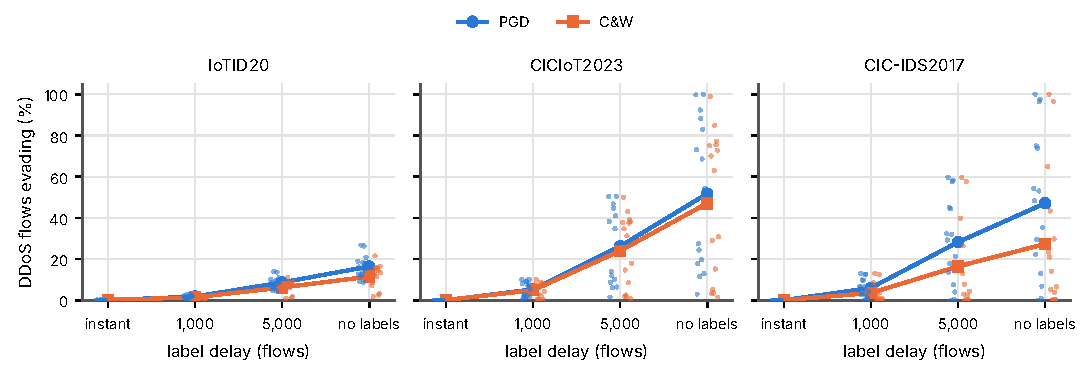
\includegraphics[width=\textwidth]{fig_label_delay.pdf}
\caption{Evasion (ASR) of PGD and C\&W transfer attacks as the label delay grows, from instant labels to no labels, for each dataset. Each dot is one seed.}
\label{fig:delay}
\end{figure*}

\subsection{Label Poisoning and Verified-Label Learning}
Verified-label learning stops poisoning, and importance weighting reduces its
false-alarm cost. Under evasion with poisoning (Fig.~\ref{fig:poison},
Table~\ref{tab:loop}), vanilla evasion grows with $q = 0.25 / 0.5 / 1$ from
3.37 to 51.50 and 99.74\% on IoTID20, and from 1.60 to 50.55 and 99.96\% on
CICIoT2023; on CIC-IDS2017 it reaches 99.95\% at $q = 1$. The failure switches
on between $q = 0.25$ and $q = 0.5$. Updating only the bandit selector (audit
policy) does not help (99.59 / 99.84 / 99.82\%), and guard is unstable at
$q = 1$ ($83.73 \pm 23.97$, $62.18 \pm 45.54$, $65.98 \pm 48.24\%$).

With a 10\% random audit budget at $q = 1$, strict (0.88 / 0.44 / 0.14\%) and
IW-strict (1.15 / 0.43 / 0.13\%) both keep evasion low
($p_{\text{Holm}} \le 0.007$ against vanilla). The cost appears in the FPR under
attack with true labels: strict raises it to 5.33 / 23.12 / 0.65\%, against
vanilla's 2.17 / 3.52 / 0.11\%, while IW-strict lowers it to 3.52 / 6.95 /
0.25\%, below strict on all three datasets ($p_{\text{Holm}} \le 0.0004$). A
20\% budget narrows the gap further (2.64 / 4.68 / 0.21\%).

\begin{figure*}[t]
\centering
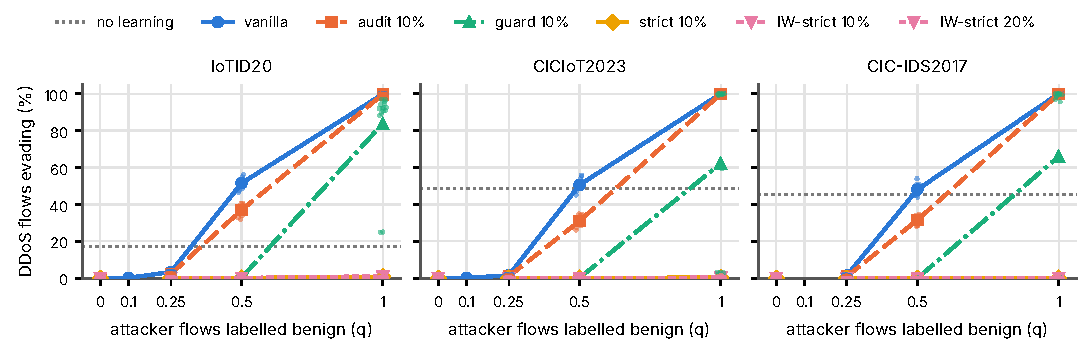
\includegraphics[width=\textwidth]{fig_loop_poison_paper.pdf}
\caption{Evasion under evasion plus label poisoning as the share $q$ of attacker flows labelled benign grows, for each update policy (10\% random audits unless stated). Dotted line: the detector without learning. Each dot is one seed.}
\label{fig:poison}
\end{figure*}

\begin{table*}[t]
\caption{Update policies under full poisoning and their cost: ASR under evasion plus poisoning ($q=1$); FPR with true labels on clean traffic and under attack. 10\% random audits unless stated; \%, mean $\pm$ std over 15 seeds. $^{\ddagger}$Identical to IW-strict: with $q=1$ no unverified DDoS label reaches the learner, so the consensus check never applies.}
\label{tab:loop}
\centering
\footnotesize
\setlength{\tabcolsep}{3pt}
\begin{tabular}{@{}lccccccccc@{}}
\toprule
 & \multicolumn{3}{c}{IoTID20} & \multicolumn{3}{c}{CICIoT2023} & \multicolumn{3}{c}{CIC-IDS2017} \\
\cmidrule(lr){2-4}\cmidrule(lr){5-7}\cmidrule(l){8-10}
Policy & ASR & FPR clean & FPR attack & ASR & FPR clean & FPR attack & ASR & FPR clean & FPR attack \\
\midrule
No labels (frozen) & 17.32$\pm$4.22 & 3.28$\pm$0.70 & 3.28$\pm$0.70 & 48.52$\pm$39.02 & 6.41$\pm$2.55 & 6.41$\pm$2.55 & 45.36$\pm$34.10 & 0.21$\pm$0.20 & 0.21$\pm$0.20 \\
Vanilla (base paper) & 99.74$\pm$0.08 & 3.33$\pm$0.63 & 2.17$\pm$0.69 & 99.96$\pm$0.03 & 5.77$\pm$2.24 & 3.52$\pm$2.01 & 99.95$\pm$0.06 & 0.12$\pm$0.08 & 0.11$\pm$0.05 \\
Audit (selector only) & 99.59$\pm$0.09 & 3.31$\pm$0.65 & 2.28$\pm$0.72 & 99.84$\pm$0.11 & 6.27$\pm$2.93 & 3.88$\pm$2.31 & 99.82$\pm$0.10 & 0.12$\pm$0.10 & 0.13$\pm$0.06 \\
Guard & 83.73$\pm$23.97 & 3.75$\pm$0.77 & 2.41$\pm$0.91 & 62.18$\pm$45.54 & 6.91$\pm$3.56 & 6.15$\pm$4.37 & 65.98$\pm$48.24 & 0.20$\pm$0.18 & 0.16$\pm$0.11 \\
Strict & 0.88$\pm$0.29 & 4.53$\pm$1.06 & 5.33$\pm$1.78 & 0.44$\pm$0.22 & 12.61$\pm$4.12 & 23.12$\pm$15.26 & 0.14$\pm$0.15 & 0.39$\pm$0.27 & 0.65$\pm$0.30 \\
IW-strict & 1.15$\pm$0.28 & 4.21$\pm$0.89 & 3.52$\pm$0.74 & 0.43$\pm$0.23 & 10.25$\pm$4.74 & 6.95$\pm$3.17 & 0.13$\pm$0.15 & 0.27$\pm$0.21 & 0.25$\pm$0.18 \\
IW-strict, 20\% audits & 0.53$\pm$0.18 & 3.95$\pm$0.64 & 2.64$\pm$0.70 & 0.30$\pm$0.14 & 7.47$\pm$2.84 & 4.68$\pm$2.45 & 0.06$\pm$0.05 & 0.16$\pm$0.13 & 0.21$\pm$0.14 \\
IW-consensus & 1.15$\pm$0.28$^\ddagger$ & 4.16$\pm$0.81 & 3.86$\pm$0.98 & 0.43$\pm$0.23$^\ddagger$ & 9.13$\pm$4.21 & 7.25$\pm$3.79 & 0.13$\pm$0.15$^\ddagger$ & 0.21$\pm$0.19 & 0.25$\pm$0.17 \\
\bottomrule
\end{tabular}
\end{table*}

\subsection{Uncertainty-Directed Audits}
Directing audits at uncertain flows lowers false alarms under attack while using
fewer audits than random allocation (Table~\ref{tab:audits}): 899--911 /
897--902 / 727--818 audits, against 992 for random audits. With true labels
under attack, IW-strict's FPR falls from 3.52 to 0.45\%, from 6.95 to 0.64\%,
and from 0.25 to 0.02\% ($p_{\text{Holm}} \le 0.005$), an 8--13$\times$
reduction that also puts it below vanilla on all three datasets
($p_{\text{Holm}} \le 0.006$). Under full poisoning, evasion falls only on
IoTID20 (strict $0.88 \to 0.28\%$, IW-strict $1.15 \to 0.31\%$,
$p_{\text{Holm}} \le 0.004$); the other datasets show no significant change.

At a matched operating point that catches 99.9\% of attacks, uncertainty audits
cut IW-strict's FPR under attack from 3.92 to 0.71\% on IoTID20 and from 5.87 to
0.64\% on CICIoT2023 ($p_{\text{Holm}} \le 0.012$), and the ROC AUC rises. On
clean IoTID20 traffic the effect reverses: the FPR rises from 3.46 to 10.39\%
(vanilla 2.90\%) and the AUC falls from 99.84 to 99.75\%; mixed audits do not
remove this (10.64\%).

\begin{table*}[t]
\caption{Audit allocation with a 10\% budget. ASR under evasion plus full poisoning ($q=1$); FPR and audits used under attack with true labels; FPR at 99.9\% detection and ROC AUC under attack and on clean traffic. Random: each flow audited with probability $a$; uncert.: the most uncertain flows (Eq.~\eqref{eq:unc}); mixed: half of the budget each. Audits used are counts out of 9{,}900 test flows. $^{\ddagger}$As in Table~\ref{tab:loop}. --: not measured.}
\label{tab:audits}
\centering
\footnotesize
\setlength{\tabcolsep}{3pt}
\begin{tabular}{@{}llccccccc@{}}
\toprule
 & & \multicolumn{3}{c}{Default threshold} & \multicolumn{2}{c}{Under attack} & \multicolumn{2}{c}{Clean traffic} \\
\cmidrule(lr){3-5}\cmidrule(lr){6-7}\cmidrule(l){8-9}
Policy & Audits & ASR ($q{=}1$) & FPR attack & Audits used & FPR@99.9\% & AUC & FPR@99.9\% & AUC \\
\midrule
\multicolumn{9}{@{}l}{\textit{IoTID20}} \\
Vanilla & -- & 99.74$\pm$0.08 & 2.17$\pm$0.69 & -- & 2.18$\pm$0.85 & 99.98$\pm$0.02 & 2.90$\pm$0.74 & 99.92$\pm$0.03 \\
Strict & random & 0.88$\pm$0.29 & 5.33$\pm$1.78 & 992$\pm$41 & -- & -- & -- & -- \\
Strict & uncert. & 0.28$\pm$0.18 & 2.45$\pm$0.73 & 911$\pm$26 & -- & -- & -- & -- \\
IW-strict & random & 1.15$\pm$0.28 & 3.52$\pm$0.74 & 992$\pm$41 & 3.92$\pm$1.35 & 99.95$\pm$0.02 & 3.46$\pm$0.95 & 99.84$\pm$0.06 \\
IW-strict & uncert. & 0.31$\pm$0.15 & 0.45$\pm$0.14 & 899$\pm$37 & 0.71$\pm$0.57 & 99.99$\pm$0.01 & 10.39$\pm$3.21 & 99.75$\pm$0.09 \\
IW-strict & mixed & 0.46$\pm$0.16 & 0.58$\pm$0.14 & 932$\pm$25 & 0.77$\pm$0.21 & 99.99$\pm$0.01 & 10.64$\pm$5.61 & 99.72$\pm$0.07 \\
IW-consensus & random & 1.15$\pm$0.28$^\ddagger$ & 3.86$\pm$0.98 & 992$\pm$41 & 9.40$\pm$6.32 & 99.94$\pm$0.04 & 3.53$\pm$1.02 & 99.82$\pm$0.07 \\
IW-consensus & uncert. & 0.31$\pm$0.15$^\ddagger$ & 0.48$\pm$0.17 & 885$\pm$43 & 1.81$\pm$3.17 & 99.98$\pm$0.02 & 11.18$\pm$3.90 & 99.75$\pm$0.07 \\
\multicolumn{9}{@{}l}{\textit{CICIoT2023}} \\
Vanilla & -- & 99.96$\pm$0.03 & 3.52$\pm$2.01 & -- & 2.38$\pm$2.03 & 99.99$\pm$0.01 & 7.55$\pm$5.01 & 99.96$\pm$0.07 \\
Strict & random & 0.44$\pm$0.22 & 23.12$\pm$15.26 & 992$\pm$41 & -- & -- & -- & -- \\
Strict & uncert. & 0.45$\pm$0.41 & 3.78$\pm$2.75 & 902$\pm$43 & -- & -- & -- & -- \\
IW-strict & random & 0.43$\pm$0.23 & 6.95$\pm$3.17 & 992$\pm$41 & 5.87$\pm$5.26 & 99.98$\pm$0.01 & 8.65$\pm$8.15 & 99.93$\pm$0.10 \\
IW-strict & uncert. & 0.46$\pm$0.39 & 0.64$\pm$0.44 & 897$\pm$51 & 0.64$\pm$0.41 & 100.00$\pm$0.00 & 5.81$\pm$4.25 & 99.98$\pm$0.01 \\
IW-strict & mixed & 0.32$\pm$0.19 & 0.68$\pm$0.29 & 958$\pm$27 & 0.60$\pm$0.56 & 100.00$\pm$0.00 & 3.66$\pm$2.56 & 99.98$\pm$0.01 \\
IW-consensus & random & 0.43$\pm$0.23$^\ddagger$ & 7.25$\pm$3.79 & 992$\pm$41 & 10.91$\pm$9.04 & 99.96$\pm$0.03 & 8.69$\pm$6.38 & 99.95$\pm$0.07 \\
IW-consensus & uncert. & 0.46$\pm$0.39$^\ddagger$ & 0.84$\pm$0.52 & 912$\pm$41 & 1.58$\pm$1.29 & 99.99$\pm$0.00 & 6.11$\pm$5.88 & 99.98$\pm$0.02 \\
\multicolumn{9}{@{}l}{\textit{CIC-IDS2017}} \\
Vanilla & -- & 99.95$\pm$0.06 & 0.11$\pm$0.05 & -- & 0.01$\pm$0.02 & 100.00$\pm$0.00 & 0.00$\pm$0.00 & 99.99$\pm$0.01 \\
Strict & random & 0.14$\pm$0.15 & 0.65$\pm$0.30 & 992$\pm$41 & -- & -- & -- & -- \\
Strict & uncert. & 0.13$\pm$0.12 & 0.11$\pm$0.07 & 818$\pm$95 & -- & -- & -- & -- \\
IW-strict & random & 0.13$\pm$0.15 & 0.25$\pm$0.18 & 992$\pm$41 & 0.02$\pm$0.03 & 100.00$\pm$0.00 & 0.01$\pm$0.03 & 99.99$\pm$0.01 \\
IW-strict & uncert. & 0.12$\pm$0.13 & 0.02$\pm$0.03 & 727$\pm$127 & 0.00$\pm$0.00 & 100.00$\pm$0.00 & 0.01$\pm$0.01 & 99.99$\pm$0.01 \\
IW-strict & mixed & -- & 0.02$\pm$0.03 & 918$\pm$62 & 0.00$\pm$0.00 & 100.00$\pm$0.00 & 0.00$\pm$0.00 & 99.99$\pm$0.01 \\
IW-consensus & random & 0.13$\pm$0.15$^\ddagger$ & 0.25$\pm$0.17 & 992$\pm$41 & 0.02$\pm$0.03 & 100.00$\pm$0.00 & 0.01$\pm$0.03 & 99.99$\pm$0.01 \\
IW-consensus & uncert. & 0.12$\pm$0.13$^\ddagger$ & 0.02$\pm$0.03 & 732$\pm$107 & 0.00$\pm$0.00 & 100.00$\pm$0.00 & 0.00$\pm$0.01 & 99.99$\pm$0.01 \\
\bottomrule
\end{tabular}
\end{table*}

\subsection{Framing}
Trusting attack labels exposes strict policies to framing
(Fig.~\ref{fig:framing}). With random audits and $r = 2\%$, strict flags 61.3 /
92.3 / 22.6\% of genuine benign flows, against 11.1 / 25.5 / 2.5\% for vanilla.
Uncertainty-directed audits lower the FPR in 34 of 36 whole-stream comparisons
and in all 36 after the campaign ($p_{\text{Holm}} \le 0.012$). After a 10\%
campaign, IW-strict's FPR falls from 36.2 to 8.9\%, 43.0 to 1.6\%, and 2.5 to
0.7\%, below vanilla's 14.7 / 15.6 / 0.9\%. IW-consensus with uncertainty
audits is never significantly worse than vanilla, during or after the campaign.
CIC-IDS2017 is far less sensitive to framing: vanilla reaches 7.1\% at
$r = 10\%$, against 37--51\% on the other two datasets. Strict update rules
should therefore not be combined with trusted attack labels without a
consensus check.

\begin{figure*}[t]
\centering
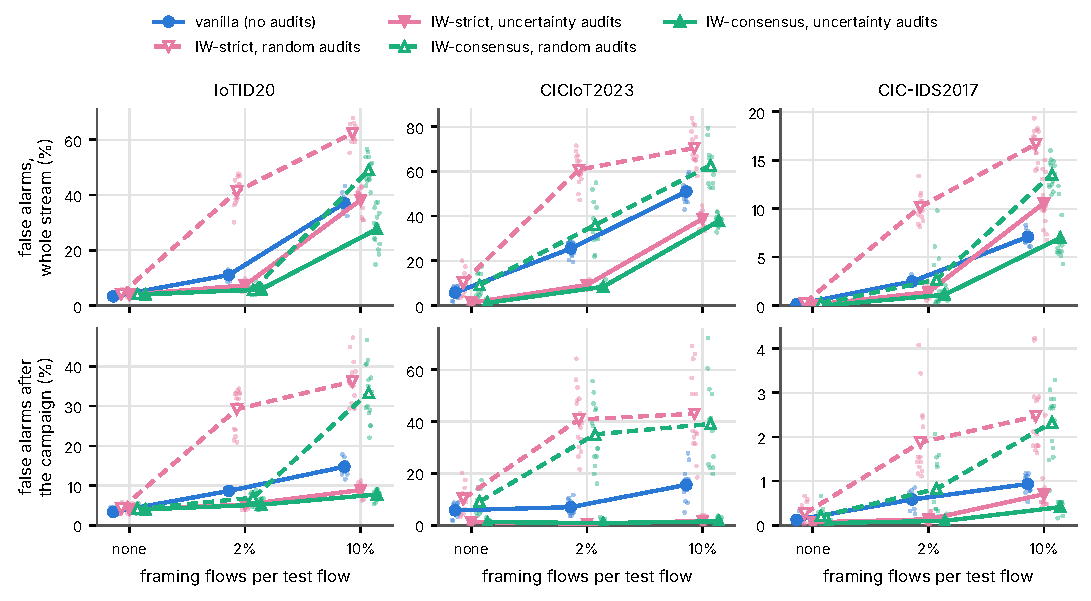
\includegraphics[width=\textwidth]{fig_framing_audits.pdf}
\caption{False alarms on genuine benign flows over the whole stream (top) and after the framing campaign (bottom) as the framing rate $r$ grows, with random and uncertainty-directed audits. Y-axis scales differ by dataset. Each dot is one seed.}
\label{fig:framing}
\end{figure*}

\subsection{The Combined Attack}
IW-consensus with uncertainty-directed audits gives the best trade-off under
the combined attack, at a measurable cost (Table~\ref{tab:combined}). With
evasion (repaired PGD), full poisoning ($q = 1$) and framing ($r = 5\%$), it
keeps the ASR at 0.65 / 0.35 / 0.15\%, while vanilla reaches 99.74 / 99.93 /
99.95\%, and its FPR of 5.23 / 13.75 / 1.95\% is below vanilla's 8.75 / 29.83 /
3.51\% ($p_{\text{Holm}} \le 0.006$). Against IW-strict, it gives lower false
alarms on all three datasets ($p_{\text{Holm}} \le 0.018$) with no significant
difference in evasion, except on CICIoT2023 (0.35 vs 0.21\%).

Without the evasion step (poisoning and framing only), IW-consensus holds the
ASR to 1.67 / 0.24 / 0.14\%, but its FPR of 11.27 / 26.07 / 2.65\% is higher
than vanilla's 7.16\% on IoTID20 (Holm-adjusted $p = 0.004$), not significantly
different on CICIoT2023 (25.01\%), and lower on CIC-IDS2017 (3.26\%). Vanilla's
lower false alarms come with 99.6--99.8\% of attacks getting through. Compared
with normal operation (the first row of each block), false alarms rise
2.4--18$\times$ with evasion and 3.4--22$\times$ without it; this is the price
of keeping evasion low.

\begin{table*}[t]
\caption{The combined attack, with and without the evasion step. ASR and FPR, \%, mean $\pm$ std over 15 seeds. The first row of each block is the undefended detector with true labels and no poisoning or framing, for reference. --: not run.}
\label{tab:combined}
\centering
\footnotesize
\setlength{\tabcolsep}{3pt}
\begin{tabular}{@{}llcccccc@{}}
\toprule
 & & \multicolumn{2}{c}{IoTID20} & \multicolumn{2}{c}{CICIoT2023} & \multicolumn{2}{c}{CIC-IDS2017} \\
\cmidrule(lr){3-4}\cmidrule(lr){5-6}\cmidrule(l){7-8}
Policy & Audits & ASR & FPR & ASR & FPR & ASR & FPR \\
\midrule
\multicolumn{8}{@{}l}{\textit{Evasion (repaired PGD) + full poisoning + 5\% framing}} \\
Vanilla, true labels & -- & 0.10$\pm$0.03 & 2.17$\pm$0.69 & 0.08$\pm$0.03 & 3.52$\pm$2.01 & 0.02$\pm$0.01 & 0.11$\pm$0.05 \\
Vanilla & -- & 99.74$\pm$0.08 & 8.75$\pm$1.67 & 99.93$\pm$0.04 & 29.83$\pm$3.98 & 99.95$\pm$0.06 & 3.51$\pm$0.31 \\
Strict & random & 0.23$\pm$0.09 & 71.63$\pm$7.75 & 0.16$\pm$0.17 & 76.28$\pm$8.44 & -- & -- \\
Strict & uncert. & 0.13$\pm$0.04 & 40.86$\pm$4.01 & 0.19$\pm$0.24 & 36.50$\pm$3.40 & 0.08$\pm$0.07 & 10.96$\pm$7.61 \\
IW-strict & random & 1.07$\pm$0.52 & 43.02$\pm$3.98 & 0.22$\pm$0.20 & 59.18$\pm$7.50 & -- & -- \\
IW-strict & uncert. & 0.58$\pm$0.19 & 17.21$\pm$4.94 & 0.21$\pm$0.24 & 17.94$\pm$2.70 & 0.12$\pm$0.10 & 3.51$\pm$1.10 \\
IW-consensus & random & 1.81$\pm$0.65 & 22.59$\pm$5.34 & 0.35$\pm$0.20 & 50.35$\pm$6.74 & -- & -- \\
IW-consensus & uncert. & 0.65$\pm$0.24 & 5.23$\pm$2.36 & 0.35$\pm$0.30 & 13.75$\pm$3.46 & 0.15$\pm$0.13 & 1.95$\pm$0.57 \\
\multicolumn{8}{@{}l}{\textit{Full poisoning + 5\% framing, no evasion}} \\
Vanilla, true labels & -- & 0.05$\pm$0.03 & 3.33$\pm$0.63 & 0.10$\pm$0.04 & 5.77$\pm$2.24 & 0.05$\pm$0.01 & 0.12$\pm$0.08 \\
Vanilla & -- & 99.61$\pm$0.05 & 7.16$\pm$1.26 & 99.72$\pm$0.04 & 25.01$\pm$3.70 & 99.84$\pm$0.04 & 3.26$\pm$0.34 \\
Strict & random & 0.19$\pm$0.18 & 73.72$\pm$4.48 & 0.02$\pm$0.03 & 82.32$\pm$6.91 & -- & -- \\
Strict & uncert. & 0.17$\pm$0.08 & 47.47$\pm$4.41 & 0.07$\pm$0.03 & 44.64$\pm$5.01 & 0.07$\pm$0.03 & 9.39$\pm$2.10 \\
IW-strict & random & 2.12$\pm$0.67 & 46.53$\pm$2.92 & 0.20$\pm$0.11 & 62.94$\pm$6.61 & -- & -- \\
IW-strict & uncert. & 1.36$\pm$0.33 & 23.85$\pm$5.62 & 0.23$\pm$0.09 & 27.91$\pm$2.36 & 0.12$\pm$0.05 & 3.26$\pm$0.72 \\
IW-consensus & random & 2.34$\pm$0.54 & 22.05$\pm$4.67 & 0.25$\pm$0.17 & 52.89$\pm$7.71 & -- & -- \\
IW-consensus & uncert. & 1.67$\pm$0.51 & 11.27$\pm$4.86 & 0.24$\pm$0.06 & 26.07$\pm$2.78 & 0.14$\pm$0.06 & 2.65$\pm$0.89 \\
\bottomrule
\end{tabular}
\end{table*}

\subsection{RADP and Adversarial Training}
On IoTID20, MSAAD's RADP filter mostly catches the impossible values of raw
attacks rather than the attacks themselves (Table~\ref{tab:baselines}, 5
seeds). It flags only 10.9--17.1\% of repaired attacks, against 91.4--100.0\% of
raw ones, so end-to-end evasion falls only from 15.96 to 12.98\%. On
CICIoT2023 it catches 98.0--99.8\% of repaired attacks but deletes 26.36\% of
genuine benign flows. Separately, perturbing every flow, as the base paper
does, produces FPRs of 65.12 / 78.38\% (IoTID20 / CICIoT2023, 3 seeds), which
explains the precision collapse reported there.

Adversarial training (15 seeds) stops transfer evasion on CICIoT2023 (48.52
$\to$ 0.03\%) but more than doubles the clean FPR (6.41 $\to$ 14.13\%,
$p_{\text{Holm}} \le 0.003$). Label-only HopSkipJump on valid traffic (5 seeds)
still evades 25.20 / 51.20\% of attacks against the plain detector and 14.00 /
2.00\% against the adversarially trained one (IoTID20 / CICIoT2023).

\begin{table}[t]
\caption{Baselines: RADP with the detector frozen, perturbing every flow, adversarial training (AT) and label-only HopSkipJump. Values in \%; RADP flag ranges are minimum--maximum over the four attacks (FGSM, BIM, PGD, C\&W); the number of seeds is given per block. --: not run.}
\label{tab:baselines}
\centering
\footnotesize
\setlength{\tabcolsep}{2.5pt}
\begin{tabular}{@{}lccc@{}}
\toprule
Measure & IoTID20 & CICIoT2023 & CIC-IDS2017 \\
\midrule
\multicolumn{4}{@{}l}{\textit{RADP, our rebuild (5 seeds; ASR on repaired PGD)}} \\
Repaired DDoS flagged & 10.9--17.1 & 98.0--99.8 & -- \\
Raw DDoS flagged & 91.4--100.0 & 98.6--100.0 & -- \\
Benign flows deleted & 0.08$\pm$0.11 & 26.36$\pm$17.15 & -- \\
ASR, w/o$\to$with RADP & 15.96$\to$12.98 & 56.23$\to$0.51 & -- \\
\multicolumn{4}{@{}l}{\textit{Perturbing every flow, no labels (3 seeds)}} \\
FPR & 65.12$\pm$11.71 & 78.38$\pm$9.55 & -- \\
\multicolumn{4}{@{}l}{\textit{Adversarial training, no labels (15 seeds; repaired PGD)}} \\
ASR, plain$\to$AT & 17.32$\to$0.12 & 48.52$\to$0.03 & 45.36$\to$0.05 \\
FPR, plain$\to$AT & 3.28$\to$5.49 & 6.41$\to$14.13 & 0.21$\to$0.96 \\
\multicolumn{4}{@{}l}{\textit{HopSkipJump, valid traffic (5 seeds)}} \\
ASR, plain / AT & 25.20 / 14.00 & 51.20 / 2.00 & -- \\
\bottomrule
\end{tabular}
\end{table}

\subsection{Detector Chain}
Adding an online MLP stage after the ensemble cuts no-label evasion on
CICIoT2023 from 48.52 to 1.93\%, but raises the FPR from 6.41 to 10.41\%. A
host-graph GNN stage is never significantly better than a parameter-matched
host-feature MLP after Holm correction. Spoofing 10 source identities raises
evasion after the full chain from 12.47 to 18.89\% on IoTID20 (campaign order)
and from 1.31 to 17.81\% on CIC-IDS2017. For DDoS from few attacker hosts,
simple per-host aggregates match message passing.

\section{Discussion and Limitations}\label{sec:discussion}

An online detector's resistance to evasion is a property of its label channel,
not only of its model. MSAAD resists evasion because its evaluation assumes an
instant, error-free feedback loop; without labels, evasion rises to 17--49\%,
and delayed labels let 9--28\% through. Any security evaluation of an adaptive
online defence should state how labels arrive and test the detector with late,
missing and poisoned labels.

Verified-label learning trades a modest audit budget for resilience to
poisoning. Directing audits at uncertain flows makes this trade cheaper under
attack: it uses fewer audits and cuts false alarms 8--13$\times$.

Trusting only one label direction opens the door to the opposite attack. For
example, strict updates stop poisoning but allow framing to succeed. While
consensus updates combined with uncertainty audits limit both threats, a
combined attack still pushes false alarms up to 2--26\%.

If you deploy this system, we advise using IW-consensus with uncertainty audits
backed by roughly a 10\% budget. For smaller budgets, copy caps help by cutting
false alarms about in half compared with a strict update strategy at a 5\%
budget. However, at a 2\% audit budget, evasion climbs to 1.8--4.0\%. Operators
should expect more false alarms during an active poisoning and framing
campaign.

Our findings have several limits. On the data side, we relied on laboratory
captures with few attacker hosts and used flow features without packet replay;
CIC-IDS2017 sits near a performance ceiling, and CICIoT2023 provides only about
330 benign test flows. Our attacker is a grey-box surrogate, not an adaptive
adversary that targets the audit rule~\cite{zhi2025ala}, and we treat a
poisoning rate of $q = 1$ as a worst case. Finally, our seeds vary
initializations, attacks and audit draws rather than the data sample itself, we
use fixed copies instead of $1/p$ weights, the false-alarm increase on clean
IoTID20 traffic is still unexplained, and MSAAD and RADP are our own
reimplementations, with only 5 seeds for the RADP and HopSkipJump experiments.

All datasets are public, and the configuration, seeds and code for every run
are available from the author.

\section{Conclusion and Future Work}\label{sec:conclusion}

This work shows that an online detector cannot adapt safely without checking
its incoming labels, and that verification should go where the model's
confidence is lowest. Instant ground-truth labels keep evasion at or below
0.12\%, but omitting or delaying them lets up to 49\% of attack flows through.
Even under simultaneous poisoning and framing, IW-consensus with
uncertainty-directed audits keeps evasion below 1.7\%, though operators must
accept a higher false-alarm rate.

We see three items for future research. First, we need to model an adaptive
attacker that targets the audit selection rule. Second, randomized audit
selection with $1/p$ weights may remove the false-alarm increase we observed
on clean traffic. Third, the system needs evaluation in real deployments with
measured label delays and packet-level replay.

\bibliographystyle{IEEEtran}
\bibliography{references}

\end{document}
